% !TeX root = ../../Report.tex
% !TeX encoding = UTF-8

در این قسمت تمام عملیات‌های پردازش درخواست‌ها شامل ثبت، ویرایش و ... کنترل می‌شوند.

\begin{figure}[H]
	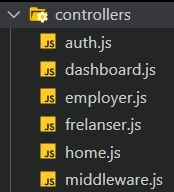
\includegraphics[width=.3\textwidth]{Folders-Files/controllers/controllers.png}
	\centering
	\caption{ساختار پوشه کنترل}
	\label{fig:folder:controllers}
\end{figure}

\subsection{فایل middleware}
در این فایل به میان‌افزارهای کنترل‌ مانند کنترل سطح دسترسی کاربر، کنترل ورود کاربر و ... پرداخته شده است.

\paragraph{\rl{logInChecker}:}
اعتبارسنجی ورود کاربر به سایت.
\\
\textbf{توضیحات}
\hr
\begin{flushleft}
	\framebox[.9\textwidth][l]{
		\lr{
			\textcolor{type}{void}
			\textcolor{func}{logInChecker}
			\textcolor{symb}{(}
			\textcolor{type}{object}
			\textcolor{arg}{request}
			\textcolor{symb}{,}
			\textcolor{type}{object}
			\textcolor{arg}{response}
			\textcolor{symb}{,}
			\textcolor{type}{object}
			\textcolor{arg}{next}
			\textcolor{symb}{);}
		}
	}
\end{flushleft}
بررسی طلاعات و ورود کاربر.
\\
\textbf{پارامترها}
\hr \\[10pt]
\begin{tabular}{|m{4cm}|m{3cm}|m{10cm}|}
	\hline
	\multicolumn{1}{|c}{پارامتر}
	&
	\multicolumn{1}{|c}{نوع}
	&
	\multicolumn{1}{|c|}{توضیحات}
	\\
	\hline
	\multicolumn{1}{|c}{request}
	&
	\multicolumn{1}{|c|}{object}
	&
	نمایانگر درخواست HTTP و دارای خصوصیاتی برای درخواست رشته پرس‌و‌جو، پارامترها ، بدنه ، هدرهای HTTP و غیره است.
	در این اسناد و طبق قرارداد ، از این شی همیشه به عنوان req یاد می شود (و پاسخ HTTP res است).
	\\
	\hline
	\multicolumn{1}{|c}{response}
	&
	\multicolumn{1}{|c|}{object}
	&
	نمایانگر پاسخ HTTP که برنامه Express با دریافت درخواست HTTP ارسال می کند.
	در این اسناد و طبق قرارداد ، از شی همیشه به عنوان res یاد می شود (و درخواست HTTP req است).
	\\
	\hline
	\multicolumn{1}{|c}{next}
	&
	\multicolumn{1}{|c|}{object}
	&
 میان‌افزار بعدی را اجرا می‌کند.
	\\
	\hline
\end{tabular}
\\[10pt]
\textbf{خروجی}
\hr \\
در صورتی که کاربر به سایت وارد شده باشد، برنامه ادامه می‌یابد، در غیر این صورت به صفحه ورود به سایت هدایت می‌شود.

\paragraph{\rl{sessionChecker}:}
اعتبارسنجی نشست‌های برنامه.
\\
\textbf{توضیحات}
\hr
\begin{flushleft}
	\framebox[.9\textwidth][l]{
		\lr{
			\textcolor{type}{void}
			\textcolor{func}{sessionChecker}
			\textcolor{symb}{(}
			\textcolor{type}{object}
			\textcolor{arg}{request}
			\textcolor{symb}{,}
			\textcolor{type}{object}
			\textcolor{arg}{response}
			\textcolor{symb}{,}
			\textcolor{type}{object}
			\textcolor{arg}{next}
			\textcolor{symb}{);}
		}
	}
\end{flushleft}
بررسی اعتبار زمانی.
\\
\textbf{پارامترها}
\hr \\[10pt]
\begin{tabular}{|m{4cm}|m{3cm}|m{10cm}|}
	\hline
	\multicolumn{1}{|c}{پارامتر}
	&
	\multicolumn{1}{|c}{نوع}
	&
	\multicolumn{1}{|c|}{توضیحات}
	\\
	\hline
	\multicolumn{1}{|c}{request}
	&
	\multicolumn{1}{|c|}{object}
	&
	نمایانگر درخواست HTTP و دارای خصوصیاتی برای درخواست رشته پرس‌و‌جو، پارامترها ، بدنه ، هدرهای HTTP و غیره است.
	در این اسناد و طبق قرارداد ، از این شی همیشه به عنوان req یاد می شود (و پاسخ HTTP res است).
	\\
	\hline
	\multicolumn{1}{|c}{response}
	&
	\multicolumn{1}{|c|}{object}
	&
	نمایانگر پاسخ HTTP که برنامه Express با دریافت درخواست HTTP ارسال می کند.
	در این اسناد و طبق قرارداد ، از شی همیشه به عنوان res یاد می شود (و درخواست HTTP req است).
	\\
	\hline
	\multicolumn{1}{|c}{next}
	&
	\multicolumn{1}{|c|}{object}
	&
 میان‌افزار بعدی را اجرا می‌کند.
	\\
	\hline
\end{tabular}
\\[10pt]
\textbf{خروجی}
\hr \\
در صورتی که مهلت زمانی ورود کاربر به پایان نرسیده باشد برنامه ادامه می‌یابد، در غیر این صورت به صفحه ورود به سایت هدایت می‌شود.

\paragraph{\rl{roleChecker}:}
اعتبارسنجی سطح دسترسی کاربر به محتوای برنامه.
\\
\textbf{توضیحات}
\hr
\begin{flushleft}
	\framebox[.9\textwidth][l]{
		\lr{
			\textcolor{type}{void}
			\textcolor{func}{logInChecker}
			\textcolor{symb}{(}
			\textcolor{type}{object}
			\textcolor{arg}{request}
			\textcolor{symb}{,}
			\textcolor{type}{object}
			\textcolor{arg}{response}
			\textcolor{symb}{,}
			\textcolor{type}{object}
			\textcolor{arg}{next}
			\textcolor{symb}{);}
		}
	}
\end{flushleft}
اعتبارسنجی سطح دسترسی کاربر.
\\
\textbf{پارامترها}
\hr \\[10pt]
\begin{tabular}{|m{4cm}|m{3cm}|m{10cm}|}
	\hline
	\multicolumn{1}{|c}{پارامتر}
	&
	\multicolumn{1}{|c}{نوع}
	&
	\multicolumn{1}{|c|}{توضیحات}
	\\
	\hline
	\multicolumn{1}{|c}{request}
	&
	\multicolumn{1}{|c|}{object}
	&
	نمایانگر درخواست HTTP و دارای خصوصیاتی برای درخواست رشته پرس‌و‌جو، پارامترها ، بدنه ، هدرهای HTTP و غیره است.
	در این اسناد و طبق قرارداد ، از این شی همیشه به عنوان req یاد می شود (و پاسخ HTTP res است).
	\\
	\hline
	\multicolumn{1}{|c}{response}
	&
	\multicolumn{1}{|c|}{object}
	&
	نمایانگر پاسخ HTTP که برنامه Express با دریافت درخواست HTTP ارسال می کند.
	در این اسناد و طبق قرارداد ، از شی همیشه به عنوان res یاد می شود (و درخواست HTTP req است).
	\\
	\hline
	\multicolumn{1}{|c}{next}
	&
	\multicolumn{1}{|c|}{object}
	&
 میان‌افزار بعدی را اجرا می‌کند.
	\\
	\hline
\end{tabular}
\\[10pt]
\textbf{خروجی}
\hr \\
در صورتی که سطح دسترسی کاربر مجار باشد برنامه ادامه می‌یابد، در غیر این صورت به صفحه قبل از درخواست هدایت می‌شود.

\subsection{فایل auth}
در این فایل به کنترل عملیات‌های احرازهویت پرداخته شده است.

\paragraph{\rl{getRegister}:}
اطلاعات صفحه ثبت‌نام را بارگذاری می‌کند.
\\
\textbf{توضیحات}
\hr
\begin{flushleft}
	\framebox[.9\textwidth][l]{
		\lr{
			\textcolor{type}{void}
			\textcolor{func}{getRegister}
			\textcolor{symb}{(}
			\textcolor{type}{object}
			\textcolor{arg}{request}
			\textcolor{symb}{,}
			\textcolor{type}{object}
			\textcolor{arg}{response}
			\textcolor{symb}{);}
		}
	}
\end{flushleft}
بارگذاری صفحه ثبت‌نام. 
\\
\textbf{پارامترها}
\hr \\[10pt]
\begin{tabular}{|m{4cm}|m{3cm}|m{10cm}|}
	\hline
	\multicolumn{1}{|c}{پارامتر}
	&
	\multicolumn{1}{|c}{نوع}
	&
	\multicolumn{1}{|c|}{توضیحات}
	\\
	\hline
	\multicolumn{1}{|c}{request}
	&
	\multicolumn{1}{|c|}{object}
	&
	نمایانگر درخواست HTTP و دارای خصوصیاتی برای درخواست رشته پرس‌و‌جو، پارامترها ، بدنه ، هدرهای HTTP و غیره است.
	در این اسناد و طبق قرارداد ، از این شی همیشه به عنوان req یاد می شود (و پاسخ HTTP res است).
	\\
	\hline
	\multicolumn{1}{|c}{response}
	&
	\multicolumn{1}{|c|}{object}
	&
	نمایانگر پاسخ HTTP که برنامه Express با دریافت درخواست HTTP ارسال می کند.
	در این اسناد و طبق قرارداد ، از شی همیشه به عنوان res یاد می شود (و درخواست HTTP req است).
	\\
	\hline
\end{tabular}
\\[10pt]
\textbf{خروجی}
\hr \\
بارگذاری اطلاعات صفحه ثبت‌نام کاربر. 

\paragraph{\rl{postRegister}:}
ثبت اطلاعات کاربر در بانک اطلاعات
\\
\textbf{توضیحات}
\hr
\begin{flushleft}
	\framebox[.9\textwidth][l]{
		\lr{
			\textcolor{type}{void}
			\textcolor{func}{postRegister}
			\textcolor{symb}{(}
			\textcolor{type}{object}
			\textcolor{arg}{request}
			\textcolor{symb}{,}
			\textcolor{type}{object}
			\textcolor{arg}{response}
			\textcolor{symb}{);}
		}
	}
\end{flushleft}
ثبت اطلاعات کاربر در پایگاه‌داده به عبارت دیگر ایجاد کاربر جدید
\\
\textbf{پارامترها}
\hr \\[10pt]
\begin{tabular}{|m{4cm}|m{3cm}|m{10cm}|}
	\hline
	\multicolumn{1}{|c}{پارامتر}
	&
	\multicolumn{1}{|c}{نوع}
	&
	\multicolumn{1}{|c|}{توضیحات}
	\\
	\hline
	\multicolumn{1}{|c}{request}
	&
	\multicolumn{1}{|c|}{object}
	&
	نمایانگر درخواست HTTP و دارای خصوصیاتی برای درخواست رشته پرس‌و‌جو، پارامترها ، بدنه ، هدرهای HTTP و غیره است.
	در این اسناد و طبق قرارداد ، از این شی همیشه به عنوان req یاد می شود (و پاسخ HTTP res است).
	\\
	\hline
	\multicolumn{1}{|c}{response}
	&
	\multicolumn{1}{|c|}{object}
	&
	نمایانگر پاسخ HTTP که برنامه Express با دریافت درخواست HTTP ارسال می کند.
	در این اسناد و طبق قرارداد ، از شی همیشه به عنوان res یاد می شود (و درخواست HTTP req است).
	\\
	\hline
\end{tabular}
\\[10pt]
\textbf{خروجی}
\hr \\
در صورت موجود نبودن کاربری کاربری جدید ایجاد می‌شود و در غیر این صورت به صفحه ورود ارجاع داده می‌شود.

\paragraph{\rl{getLogIn}:}
اطلاعات صفحه ورود را بارگذاری می‌کند.
\\
\textbf{توضیحات}
\hr
\begin{flushleft}
	\framebox[.9\textwidth][l]{
		\lr{
			\textcolor{type}{void}
			\textcolor{func}{getLogIn}
			\textcolor{symb}{(}
			\textcolor{type}{object}
			\textcolor{arg}{request}
			\textcolor{symb}{,}
			\textcolor{type}{object}
			\textcolor{arg}{response}
			\textcolor{symb}{);}
		}
	}
\end{flushleft}
هر کاربر با درج اطلاعات صحیح خود با شناسه‌ای یکتا به برنامه وارد می‌شود.
\\
\textbf{پارامترها}
\hr \\[10pt]
\begin{tabular}{|m{4cm}|m{3cm}|m{10cm}|}
	\hline
	\multicolumn{1}{|c}{پارامتر}
	&
	\multicolumn{1}{|c}{نوع}
	&
	\multicolumn{1}{|c|}{توضیحات}
	\\
	\hline
	\multicolumn{1}{|c}{request}
	&
	\multicolumn{1}{|c|}{object}
	&
	نمایانگر درخواست HTTP و دارای خصوصیاتی برای درخواست رشته پرس‌و‌جو، پارامترها ، بدنه ، هدرهای HTTP و غیره است.
	در این اسناد و طبق قرارداد ، از این شی همیشه به عنوان req یاد می شود (و پاسخ HTTP res است).
	\\
	\hline
	\multicolumn{1}{|c}{response}
	&
	\multicolumn{1}{|c|}{object}
	&
	نمایانگر پاسخ HTTP که برنامه Express با دریافت درخواست HTTP ارسال می کند.
	در این اسناد و طبق قرارداد ، از شی همیشه به عنوان res یاد می شود (و درخواست HTTP req است).
	\\
	\hline
\end{tabular}
\\[10pt]
\textbf{خروجی}
\hr \\
در صورت موجود بودن کاربری به برنامه وارد می‌شود و در غیراین‌صورت به صفحه ثبت‌نام ارجاع داده می‌شود.

\paragraph{\rl{postLogIn}:}
دریافت اطلاعات کاربر از بانک اطلاعات
\\
\textbf{توضیحات}
\hr
\begin{flushleft}
	\framebox[.9\textwidth][l]{
		\lr{
			\textcolor{type}{void}
			\textcolor{func}{postLogIn}
			\textcolor{symb}{(}
			\textcolor{type}{object}
			\textcolor{arg}{request}
			\textcolor{symb}{,}
			\textcolor{type}{object}
			\textcolor{arg}{response}
			\textcolor{symb}{);}
		}
	}
\end{flushleft}
دریافت اطلاعات کاربر از پایگاه‌داده و ورود به برنامه
\\
\textbf{پارامترها}
\hr \\[10pt]
\begin{tabular}{|m{4cm}|m{3cm}|m{10cm}|}
	\hline
	\multicolumn{1}{|c}{پارامتر}
	&
	\multicolumn{1}{|c}{نوع}
	&
	\multicolumn{1}{|c|}{توضیحات}
	\\
	\hline
	\multicolumn{1}{|c}{request}
	&
	\multicolumn{1}{|c|}{object}
	&
	نمایانگر درخواست HTTP و دارای خصوصیاتی برای درخواست رشته پرس‌و‌جو، پارامترها ، بدنه ، هدرهای HTTP و غیره است.
	در این اسناد و طبق قرارداد ، از این شی همیشه به عنوان req یاد می شود (و پاسخ HTTP res است).
	\\
	\hline
	\multicolumn{1}{|c}{response}
	&
	\multicolumn{1}{|c|}{object}
	&
	نمایانگر پاسخ HTTP که برنامه Express با دریافت درخواست HTTP ارسال می کند.
	در این اسناد و طبق قرارداد ، از شی همیشه به عنوان res یاد می شود (و درخواست HTTP req است).
	\\
	\hline
\end{tabular}
\\[10pt]
\textbf{خروجی}
\hr \\
در صورت موجود بودن کاربر به صفحه داشبورد ارجاع داده می‌شود و در غیر این صورت به صفحه ثبت‌نام ارجاع داده می‌شود.


\paragraph{\rl{getForgot}:}
فراموشی رمز عبور
\\
\textbf{توضیحات}
\hr
\begin{flushleft}
	\framebox[.9\textwidth][l]{
		\lr{
			\textcolor{type}{void}
			\textcolor{func}{getForgot}
			\textcolor{symb}{(}
			\textcolor{type}{object}
			\textcolor{arg}{request}
			\textcolor{symb}{,}
			\textcolor{type}{object}
			\textcolor{arg}{response}
			\textcolor{symb}{);}
		}
	}
\end{flushleft}
صفحه فراموشی رمز عبور را بارگذاری می‌کند.
\\
\textbf{پارامترها}
\hr \\[10pt]
\begin{tabular}{|m{4cm}|m{3cm}|m{10cm}|}
	\hline
	\multicolumn{1}{|c}{پارامتر}
	&
	\multicolumn{1}{|c}{نوع}
	&
	\multicolumn{1}{|c|}{توضیحات}
	\\
	\hline
	\multicolumn{1}{|c}{request}
	&
	\multicolumn{1}{|c|}{object}
	&
	نمایانگر درخواست HTTP و دارای خصوصیاتی برای درخواست رشته پرس‌و‌جو، پارامترها ، بدنه ، هدرهای HTTP و غیره است.
	در این اسناد و طبق قرارداد ، از این شی همیشه به عنوان req یاد می شود (و پاسخ HTTP res است).
	\\
	\hline
	\multicolumn{1}{|c}{response}
	&
	\multicolumn{1}{|c|}{object}
	&
	نمایانگر پاسخ HTTP که برنامه Express با دریافت درخواست HTTP ارسال می کند.
	در این اسناد و طبق قرارداد ، از شی همیشه به عنوان res یاد می شود (و درخواست HTTP req است).
	\\
	\hline
\end{tabular}
\\[10pt]
\textbf{خروجی}
\hr \\
بارگذاری صفحه فراموشی رمز عبور.


\paragraph{\rl{postForgot}:}
دریافت اطلاعات کاربر از بانک اطلاعات
\\
\textbf{توضیحات}
\hr
\begin{flushleft}
	\framebox[.9\textwidth][l]{
		\lr{
			\textcolor{type}{void}
			\textcolor{func}{postForgot}
			\textcolor{symb}{(}
			\textcolor{type}{object}
			\textcolor{arg}{request}
			\textcolor{symb}{,}
			\textcolor{type}{object}
			\textcolor{arg}{response}
			\textcolor{symb}{);}
		}
	}
\end{flushleft}
دریافت اطلاعات کاربر از پایگاه‌داده و ورود به مرحله بازیابی رمز عبور.
\\
\textbf{پارامترها}
\hr \\[10pt]
\begin{tabular}{|m{4cm}|m{3cm}|m{10cm}|}
	\hline
	\multicolumn{1}{|c}{پارامتر}
	&
	\multicolumn{1}{|c}{نوع}
	&
	\multicolumn{1}{|c|}{توضیحات}
	\\
	\hline
	\multicolumn{1}{|c}{request}
	&
	\multicolumn{1}{|c|}{object}
	&
	نمایانگر درخواست HTTP و دارای خصوصیاتی برای درخواست رشته پرس‌و‌جو، پارامترها ، بدنه ، هدرهای HTTP و غیره است.
	در این اسناد و طبق قرارداد ، از این شی همیشه به عنوان req یاد می شود (و پاسخ HTTP res است).
	\\
	\hline
	\multicolumn{1}{|c}{response}
	&
	\multicolumn{1}{|c|}{object}
	&
	نمایانگر پاسخ HTTP که برنامه Express با دریافت درخواست HTTP ارسال می کند.
	در این اسناد و طبق قرارداد ، از شی همیشه به عنوان res یاد می شود (و درخواست HTTP req است).
	\\
	\hline
\end{tabular}
\\[10pt]
\textbf{خروجی}
\hr \\
در صورت موجود بودن کاربری به صفحه بازیابی اطلاعات ارجاع داده می‌شود، در غیراین‌صورت به صفحه ثبت‌نام ارجاع داده می‌شود.

\paragraph{\rl{getRecover}:}
بازیابی رمز عبور
\\
\textbf{توضیحات}
\hr
\begin{flushleft}
	\framebox[.9\textwidth][l]{
		\lr{
			\textcolor{type}{void}
			\textcolor{func}{getRecover}
			\textcolor{symb}{(}
			\textcolor{type}{object}
			\textcolor{arg}{request}
			\textcolor{symb}{,}
			\textcolor{type}{object}
			\textcolor{arg}{response}
			\textcolor{symb}{);}
		}
	}
\end{flushleft}
صفحه بازیابی رمز عبور را بارگذاری و توکن ارسال شده به پست الکترونیک کاربر را اعتبار سنجی می‌کند.
\\
\textbf{پارامترها}
\hr \\[10pt]
\begin{tabular}{|m{4cm}|m{3cm}|m{10cm}|}
	\hline
	\multicolumn{1}{|c}{پارامتر}
	&
	\multicolumn{1}{|c}{نوع}
	&
	\multicolumn{1}{|c|}{توضیحات}
	\\
	\hline
	\multicolumn{1}{|c}{request}
	&
	\multicolumn{1}{|c|}{object}
	&
	نمایانگر درخواست HTTP و دارای خصوصیاتی برای درخواست رشته پرس‌و‌جو، پارامترها ، بدنه ، هدرهای HTTP و غیره است.
	در این اسناد و طبق قرارداد ، از این شی همیشه به عنوان req یاد می شود (و پاسخ HTTP res است).
	\\
	\hline
	\multicolumn{1}{|c}{response}
	&
	\multicolumn{1}{|c|}{object}
	&
	نمایانگر پاسخ HTTP که برنامه Express با دریافت درخواست HTTP ارسال می کند.
	در این اسناد و طبق قرارداد ، از شی همیشه به عنوان res یاد می شود (و درخواست HTTP req است).
	\\
	\hline
\end{tabular}
\\[10pt]
\textbf{خروجی}
\hr \\
درصورت صحت توکن کاربر  صفحه بازیابی رمز عبور را بارگذاری می‌کند.


\paragraph{\rl{postRecover}:}
ویزایش اطلاعات کاربری بازیابی شده
\\
\textbf{توضیحات}
\hr
\begin{flushleft}
	\framebox[.9\textwidth][l]{
		\lr{
			\textcolor{type}{void}
			\textcolor{func}{postRecover}
			\textcolor{symb}{(}
			\textcolor{type}{object}
			\textcolor{arg}{request}
			\textcolor{symb}{,}
			\textcolor{type}{object}
			\textcolor{arg}{response}
			\textcolor{symb}{);}
		}
	}
\end{flushleft}
ویزایش اطلاعات کاربری بازیابی شده در بانک اطلاعات
\\
\textbf{پارامترها}
\hr \\[10pt]
\begin{tabular}{|m{4cm}|m{3cm}|m{10cm}|}
	\hline
	\multicolumn{1}{|c}{پارامتر}
	&
	\multicolumn{1}{|c}{نوع}
	&
	\multicolumn{1}{|c|}{توضیحات}
	\\
	\hline
	\multicolumn{1}{|c}{request}
	&
	\multicolumn{1}{|c|}{object}
	&
	نمایانگر درخواست HTTP و دارای خصوصیاتی برای درخواست رشته پرس‌و‌جو، پارامترها ، بدنه ، هدرهای HTTP و غیره است.
	در این اسناد و طبق قرارداد ، از این شی همیشه به عنوان req یاد می شود (و پاسخ HTTP res است).
	\\
	\hline
	\multicolumn{1}{|c}{response}
	&
	\multicolumn{1}{|c|}{object}
	&
	نمایانگر پاسخ HTTP که برنامه Express با دریافت درخواست HTTP ارسال می کند.
	در این اسناد و طبق قرارداد ، از شی همیشه به عنوان res یاد می شود (و درخواست HTTP req است).
	\\
	\hline
\end{tabular}
\\[10pt]
\textbf{خروجی}
\hr \\
اطلاعات کاربر بازیابی شده و به صفحه داشبورد ارجاع داده می‌شود.


\subsection{فایل employer}
در این فایل به کنترل تمام عملیات‌های داشبورد کارفرما پرداخته شده است.

\paragraph{\rl{getRoot}:}
داشبورد کارفرما
\\
\textbf{توضیحات}
\hr
\begin{flushleft}
	\framebox[.9\textwidth][l]{
		\lr{
			\textcolor{type}{void}
			\textcolor{func}{getRoot}
			\textcolor{symb}{(}
			\textcolor{type}{object}
			\textcolor{arg}{request}
			\textcolor{symb}{,}
			\textcolor{type}{object}
			\textcolor{arg}{response}
			\textcolor{symb}{);}
		}
	}
\end{flushleft}
صفحه داشبورد کارفرما را بارگذاری می‌کند.
\\
\textbf{پارامترها}
\hr \\[10pt]
\begin{tabular}{|m{4cm}|m{3cm}|m{10cm}|}
	\hline
	\multicolumn{1}{|c}{پارامتر}
	&
	\multicolumn{1}{|c}{نوع}
	&
	\multicolumn{1}{|c|}{توضیحات}
	\\
	\hline
	\multicolumn{1}{|c}{request}
	&
	\multicolumn{1}{|c|}{object}
	&
	نمایانگر درخواست HTTP و دارای خصوصیاتی برای درخواست رشته پرس‌و‌جو، پارامترها ، بدنه ، هدرهای HTTP و غیره است.
	در این اسناد و طبق قرارداد ، از این شی همیشه به عنوان req یاد می شود (و پاسخ HTTP res است).
	\\
	\hline
	\multicolumn{1}{|c}{response}
	&
	\multicolumn{1}{|c|}{object}
	&
	نمایانگر پاسخ HTTP که برنامه Express با دریافت درخواست HTTP ارسال می کند.
	در این اسناد و طبق قرارداد ، از شی همیشه به عنوان res یاد می شود (و درخواست HTTP req است).
	\\
	\hline
\end{tabular}
\\[10pt]
\textbf{خروجی}
\hr \\
بارگذاری داشبورد کارفرما.


\paragraph{\rl{getProject}:}
لیست پروژه‌های کارفرما
\\
\textbf{توضیحات}
\hr
\begin{flushleft}
	\framebox[.9\textwidth][l]{
		\lr{
			\textcolor{type}{void}
			\textcolor{func}{getProject}
			\textcolor{symb}{(}
			\textcolor{type}{object}
			\textcolor{arg}{request}
			\textcolor{symb}{,}
			\textcolor{type}{object}
			\textcolor{arg}{response}
			\textcolor{symb}{);}
		}
	}
\end{flushleft}
صفحه لیست پروژه‌های کارفرما را بارگذاری می‌کند.
\\
\textbf{پارامترها}
\hr \\[10pt]
\begin{tabular}{|m{4cm}|m{3cm}|m{10cm}|}
	\hline
	\multicolumn{1}{|c}{پارامتر}
	&
	\multicolumn{1}{|c}{نوع}
	&
	\multicolumn{1}{|c|}{توضیحات}
	\\
	\hline
	\multicolumn{1}{|c}{request}
	&
	\multicolumn{1}{|c|}{object}
	&
	نمایانگر درخواست HTTP و دارای خصوصیاتی برای درخواست رشته پرس‌و‌جو، پارامترها ، بدنه ، هدرهای HTTP و غیره است.
	در این اسناد و طبق قرارداد ، از این شی همیشه به عنوان req یاد می شود (و پاسخ HTTP res است).
	\\
	\hline
	\multicolumn{1}{|c}{response}
	&
	\multicolumn{1}{|c|}{object}
	&
	نمایانگر پاسخ HTTP که برنامه Express با دریافت درخواست HTTP ارسال می کند.
	در این اسناد و طبق قرارداد ، از شی همیشه به عنوان res یاد می شود (و درخواست HTTP req است).
	\\
	\hline
\end{tabular}
\\[10pt]
\textbf{خروجی}
\hr \\
بارگذاری صفحه لیست پروژه‌های کارفرما.

\paragraph{\rl{getAddProject}:}
تعریف پروژه‌ توسط کارفرما
\\
\textbf{توضیحات}
\hr
\begin{flushleft}
	\framebox[.9\textwidth][l]{
		\lr{
			\textcolor{type}{void}
			\textcolor{func}{getAddProject}
			\textcolor{symb}{(}
			\textcolor{type}{object}
			\textcolor{arg}{request}
			\textcolor{symb}{,}
			\textcolor{type}{object}
			\textcolor{arg}{response}
			\textcolor{symb}{);}
		}
	}
\end{flushleft}
صفحه ایجاد پروژه را بارگذاری می‌کند.
\\
\textbf{پارامترها}
\hr \\[10pt]
\begin{tabular}{|m{4cm}|m{3cm}|m{10cm}|}
	\hline
	\multicolumn{1}{|c}{پارامتر}
	&
	\multicolumn{1}{|c}{نوع}
	&
	\multicolumn{1}{|c|}{توضیحات}
	\\
	\hline
	\multicolumn{1}{|c}{request}
	&
	\multicolumn{1}{|c|}{object}
	&
	نمایانگر درخواست HTTP و دارای خصوصیاتی برای درخواست رشته پرس‌و‌جو، پارامترها ، بدنه ، هدرهای HTTP و غیره است.
	در این اسناد و طبق قرارداد ، از این شی همیشه به عنوان req یاد می شود (و پاسخ HTTP res است).
	\\
	\hline
	\multicolumn{1}{|c}{response}
	&
	\multicolumn{1}{|c|}{object}
	&
	نمایانگر پاسخ HTTP که برنامه Express با دریافت درخواست HTTP ارسال می کند.
	در این اسناد و طبق قرارداد ، از شی همیشه به عنوان res یاد می شود (و درخواست HTTP req است).
	\\
	\hline
\end{tabular}
\\[10pt]
\textbf{خروجی}
\hr \\
بارگذاری صفحه ایجاد پروژه توسط کارفرما.

\paragraph{\rl{postAddProject}:}
ثبت اطلاعات پروژه در بانک اطلاعات
\\
\textbf{توضیحات}
\hr
\begin{flushleft}
	\framebox[.9\textwidth][l]{
		\lr{
			\textcolor{type}{void}
			\textcolor{func}{postAddProject}
			\textcolor{symb}{(}
			\textcolor{type}{object}
			\textcolor{arg}{request}
			\textcolor{symb}{,}
			\textcolor{type}{object}
			\textcolor{arg}{response}
			\textcolor{symb}{);}
		}
	}
\end{flushleft}
ثبت اطلاعات پروژه در پایگاه‌داده
\\
\textbf{پارامترها}
\hr \\[10pt]
\begin{tabular}{|m{4cm}|m{3cm}|m{10cm}|}
	\hline
	\multicolumn{1}{|c}{پارامتر}
	&
	\multicolumn{1}{|c}{نوع}
	&
	\multicolumn{1}{|c|}{توضیحات}
	\\
	\hline
	\multicolumn{1}{|c}{request}
	&
	\multicolumn{1}{|c|}{object}
	&
	نمایانگر درخواست HTTP و دارای خصوصیاتی برای درخواست رشته پرس‌و‌جو، پارامترها ، بدنه ، هدرهای HTTP و غیره است.
	در این اسناد و طبق قرارداد ، از این شی همیشه به عنوان req یاد می شود (و پاسخ HTTP res است).
	\\
	\hline
	\multicolumn{1}{|c}{response}
	&
	\multicolumn{1}{|c|}{object}
	&
	نمایانگر پاسخ HTTP که برنامه Express با دریافت درخواست HTTP ارسال می کند.
	در این اسناد و طبق قرارداد ، از شی همیشه به عنوان res یاد می شود (و درخواست HTTP req است).
	\\
	\hline
\end{tabular}
\\[10pt]
\textbf{خروجی}
\hr \\
اطلاعات پروژه ثبت شده و به صفحه لیست پروژه‌ها ارجاع داده می‌شود.

\paragraph{\rl{getEditProject}:}
 ویرایش پروژه‌ 
\\
\textbf{توضیحات}
\hr
\begin{flushleft}
	\framebox[.9\textwidth][l]{
		\lr{
			\textcolor{type}{void}
			\textcolor{func}{getEditProject}
			\textcolor{symb}{(}
			\textcolor{type}{object}
			\textcolor{arg}{request}
			\textcolor{symb}{,}
			\textcolor{type}{object}
			\textcolor{arg}{response}
			\textcolor{symb}{);}
		}
	}
\end{flushleft}
بارگذاری صفحه ویرایش پروژه بارگذاری می‌کند.
\\
\textbf{پارامترها}
\hr \\[10pt]
\begin{tabular}{|m{4cm}|m{3cm}|m{10cm}|}
	\hline
	\multicolumn{1}{|c}{پارامتر}
	&
	\multicolumn{1}{|c}{نوع}
	&
	\multicolumn{1}{|c|}{توضیحات}
	\\
	\hline
	\multicolumn{1}{|c}{request}
	&
	\multicolumn{1}{|c|}{object}
	&
	نمایانگر درخواست HTTP و دارای خصوصیاتی برای درخواست رشته پرس‌و‌جو، پارامترها ، بدنه ، هدرهای HTTP و غیره است.
	در این اسناد و طبق قرارداد ، از این شی همیشه به عنوان req یاد می شود (و پاسخ HTTP res است).
	\\
	\hline
	\multicolumn{1}{|c}{response}
	&
	\multicolumn{1}{|c|}{object}
	&
	نمایانگر پاسخ HTTP که برنامه Express با دریافت درخواست HTTP ارسال می کند.
	در این اسناد و طبق قرارداد ، از شی همیشه به عنوان res یاد می شود (و درخواست HTTP req است).
	\\
	\hline
\end{tabular}
\\[10pt]
\textbf{خروجی}
\hr \\
بارگذاری صفحه ویرایش پروژه توسط کارفرما.

\paragraph{\rl{postEditProject}:}
ویرایش اطلاعات پروژه در بانک اطلاعات
\\
\textbf{توضیحات}
\hr
\begin{flushleft}
	\framebox[.9\textwidth][l]{
		\lr{
			\textcolor{type}{void}
			\textcolor{func}{postEditProject}
			\textcolor{symb}{(}
			\textcolor{type}{object}
			\textcolor{arg}{request}
			\textcolor{symb}{,}
			\textcolor{type}{object}
			\textcolor{arg}{response}
			\textcolor{symb}{);}
		}
	}
\end{flushleft}
ویرایش اطلاعات پروژه در پایگاه‌داده
\\
\textbf{پارامترها}
\hr \\[10pt]
\begin{tabular}{|m{4cm}|m{3cm}|m{10cm}|}
	\hline
	\multicolumn{1}{|c}{پارامتر}
	&
	\multicolumn{1}{|c}{نوع}
	&
	\multicolumn{1}{|c|}{توضیحات}
	\\
	\hline
	\multicolumn{1}{|c}{request}
	&
	\multicolumn{1}{|c|}{object}
	&
	نمایانگر درخواست HTTP و دارای خصوصیاتی برای درخواست رشته پرس‌و‌جو، پارامترها ، بدنه ، هدرهای HTTP و غیره است.
	در این اسناد و طبق قرارداد ، از این شی همیشه به عنوان req یاد می شود (و پاسخ HTTP res است).
	\\
	\hline
	\multicolumn{1}{|c}{response}
	&
	\multicolumn{1}{|c|}{object}
	&
	نمایانگر پاسخ HTTP که برنامه Express با دریافت درخواست HTTP ارسال می کند.
	در این اسناد و طبق قرارداد ، از شی همیشه به عنوان res یاد می شود (و درخواست HTTP req است).
	\\
	\hline
\end{tabular}
\\[10pt]
\textbf{خروجی}
\hr \\
اطلاعات پروژه ویرایش شده و به صفحه لیست پروژه‌ها ارجاع داده می‌شود.

\paragraph{\rl{getDeleteProject}:}
حذف پروژه‌ 
\\
\textbf{توضیحات}
\hr
\begin{flushleft}
	\framebox[.9\textwidth][l]{
		\lr{
			\textcolor{type}{void}
			\textcolor{func}{getDeleteProject}
			\textcolor{symb}{(}
			\textcolor{type}{object}
			\textcolor{arg}{request}
			\textcolor{symb}{,}
			\textcolor{type}{object}
			\textcolor{arg}{response}
			\textcolor{symb}{);}
		}
	}
\end{flushleft}
حذف پروژه از پایگاه‌داده.
\\
\textbf{پارامترها}
\hr \\[10pt]
\begin{tabular}{|m{4cm}|m{3cm}|m{10cm}|}
	\hline
	\multicolumn{1}{|c}{پارامتر}
	&
	\multicolumn{1}{|c}{نوع}
	&
	\multicolumn{1}{|c|}{توضیحات}
	\\
	\hline
	\multicolumn{1}{|c}{request}
	&
	\multicolumn{1}{|c|}{object}
	&
	نمایانگر درخواست HTTP و دارای خصوصیاتی برای درخواست رشته پرس‌و‌جو، پارامترها ، بدنه ، هدرهای HTTP و غیره است.
	در این اسناد و طبق قرارداد ، از این شی همیشه به عنوان req یاد می شود (و پاسخ HTTP res است).
	\\
	\hline
	\multicolumn{1}{|c}{response}
	&
	\multicolumn{1}{|c|}{object}
	&
	نمایانگر پاسخ HTTP که برنامه Express با دریافت درخواست HTTP ارسال می کند.
	در این اسناد و طبق قرارداد ، از شی همیشه به عنوان res یاد می شود (و درخواست HTTP req است).
	\\
	\hline
\end{tabular}
\\[10pt]
\textbf{خروجی}
\hr \\
حذف پروژه از پایگاه‌داده توسط کارفرما.

\paragraph{\rl{getDetailProject}:}
نمایش پروژه‌ 
\\
\textbf{توضیحات}
\hr
\begin{flushleft}
	\framebox[.9\textwidth][l]{
		\lr{
			\textcolor{type}{void}
			\textcolor{func}{getDetailProject}
			\textcolor{symb}{(}
			\textcolor{type}{object}
			\textcolor{arg}{request}
			\textcolor{symb}{,}
			\textcolor{type}{object}
			\textcolor{arg}{response}
			\textcolor{symb}{);}
		}
	}
\end{flushleft}
صفحه نمایش اطلاعات پروژه بارگذاری می‌کند.
\\
\textbf{پارامترها}
\hr \\[10pt]
\begin{tabular}{|m{4cm}|m{3cm}|m{10cm}|}
	\hline
	\multicolumn{1}{|c}{پارامتر}
	&
	\multicolumn{1}{|c}{نوع}
	&
	\multicolumn{1}{|c|}{توضیحات}
	\\
	\hline
	\multicolumn{1}{|c}{request}
	&
	\multicolumn{1}{|c|}{object}
	&
	نمایانگر درخواست HTTP و دارای خصوصیاتی برای درخواست رشته پرس‌و‌جو، پارامترها ، بدنه ، هدرهای HTTP و غیره است.
	در این اسناد و طبق قرارداد ، از این شی همیشه به عنوان req یاد می شود (و پاسخ HTTP res است).
	\\
	\hline
	\multicolumn{1}{|c}{response}
	&
	\multicolumn{1}{|c|}{object}
	&
	نمایانگر پاسخ HTTP که برنامه Express با دریافت درخواست HTTP ارسال می کند.
	در این اسناد و طبق قرارداد ، از شی همیشه به عنوان res یاد می شود (و درخواست HTTP req است).
	\\
	\hline
\end{tabular}
\\[10pt]
\textbf{خروجی}
\hr \\
بارگذاری صفحه نمایش اطلاعات پروژه.

\paragraph{\rl{getInvoiceProject}:}
پرداخت هزینه پروژه
\\
\textbf{توضیحات}
\hr
\begin{flushleft}
	\framebox[.9\textwidth][l]{
		\lr{
			\textcolor{type}{void}
			\textcolor{func}{getInvoiceProject}
			\textcolor{symb}{(}
			\textcolor{type}{object}
			\textcolor{arg}{request}
			\textcolor{symb}{,}
			\textcolor{type}{object}
			\textcolor{arg}{response}
			\textcolor{symb}{);}
		}
	}
\end{flushleft}
صفحه پرداخت هزینه پروژه بارگذاری می‌کند.
\\
\textbf{پارامترها}
\hr \\[10pt]
\begin{tabular}{|m{4cm}|m{3cm}|m{10cm}|}
	\hline
	\multicolumn{1}{|c}{پارامتر}
	&
	\multicolumn{1}{|c}{نوع}
	&
	\multicolumn{1}{|c|}{توضیحات}
	\\
	\hline
	\multicolumn{1}{|c}{request}
	&
	\multicolumn{1}{|c|}{object}
	&
	نمایانگر درخواست HTTP و دارای خصوصیاتی برای درخواست رشته پرس‌و‌جو، پارامترها ، بدنه ، هدرهای HTTP و غیره است.
	در این اسناد و طبق قرارداد ، از این شی همیشه به عنوان req یاد می شود (و پاسخ HTTP res است).
	\\
	\hline
	\multicolumn{1}{|c}{response}
	&
	\multicolumn{1}{|c|}{object}
	&
	نمایانگر پاسخ HTTP که برنامه Express با دریافت درخواست HTTP ارسال می کند.
	در این اسناد و طبق قرارداد ، از شی همیشه به عنوان res یاد می شود (و درخواست HTTP req است).
	\\
	\hline
\end{tabular}
\\[10pt]
\textbf{خروجی}
\hr \\
بارگذاری صفحه پرداخت هزینه پروژه.

\paragraph{\rl{postInvoiceProject}:}
ثبت اطلاعات پرداخت هزینه پروژه در بانک اطلاعات
\\
\textbf{توضیحات}
\hr
\begin{flushleft}
	\framebox[.9\textwidth][l]{
		\lr{
			\textcolor{type}{void}
			\textcolor{func}{postInvoiceProject}
			\textcolor{symb}{(}
			\textcolor{type}{object}
			\textcolor{arg}{request}
			\textcolor{symb}{,}
			\textcolor{type}{object}
			\textcolor{arg}{response}
			\textcolor{symb}{);}
		}
	}
\end{flushleft}
ثبت اطلاعات پرداخت هزینه پروژه در پایگاه‌داده
\\
\textbf{پارامترها}
\hr \\[10pt]
\begin{tabular}{|m{4cm}|m{3cm}|m{10cm}|}
	\hline
	\multicolumn{1}{|c}{پارامتر}
	&
	\multicolumn{1}{|c}{نوع}
	&
	\multicolumn{1}{|c|}{توضیحات}
	\\
	\hline
	\multicolumn{1}{|c}{request}
	&
	\multicolumn{1}{|c|}{object}
	&
	نمایانگر درخواست HTTP و دارای خصوصیاتی برای درخواست رشته پرس‌و‌جو، پارامترها ، بدنه ، هدرهای HTTP و غیره است.
	در این اسناد و طبق قرارداد ، از این شی همیشه به عنوان req یاد می شود (و پاسخ HTTP res است).
	\\
	\hline
	\multicolumn{1}{|c}{response}
	&
	\multicolumn{1}{|c|}{object}
	&
	نمایانگر پاسخ HTTP که برنامه Express با دریافت درخواست HTTP ارسال می کند.
	در این اسناد و طبق قرارداد ، از شی همیشه به عنوان res یاد می شود (و درخواست HTTP req است).
	\\
	\hline
\end{tabular}
\\[10pt]
\textbf{خروجی}
\hr \\
ثبت اطلاعات پرداخت هزینه و انجام فرایند تسویه حساب با فریلنسر.


\subsection{فایل frelanser}
در این فایل به کنترل تمام عملیات‌های داشبورد فریلنسر پرداخته شده است.

\paragraph{\rl{getRoot}:}
داشبورد فریلنسر
\\
\textbf{توضیحات}
\hr
\begin{flushleft}
	\framebox[.9\textwidth][l]{
		\lr{
			\textcolor{type}{void}
			\textcolor{func}{getRoot}
			\textcolor{symb}{(}
			\textcolor{type}{object}
			\textcolor{arg}{request}
			\textcolor{symb}{,}
			\textcolor{type}{object}
			\textcolor{arg}{response}
			\textcolor{symb}{);}
		}
	}
\end{flushleft}
صفحه داشبورد فریلنسر را بارگذاری می‌کند.
\\
\textbf{پارامترها}
\hr \\[10pt]
\begin{tabular}{|m{4cm}|m{3cm}|m{10cm}|}
	\hline
	\multicolumn{1}{|c}{پارامتر}
	&
	\multicolumn{1}{|c}{نوع}
	&
	\multicolumn{1}{|c|}{توضیحات}
	\\
	\hline
	\multicolumn{1}{|c}{request}
	&
	\multicolumn{1}{|c|}{object}
	&
	نمایانگر درخواست HTTP و دارای خصوصیاتی برای درخواست رشته پرس‌و‌جو، پارامترها ، بدنه ، هدرهای HTTP و غیره است.
	در این اسناد و طبق قرارداد ، از این شی همیشه به عنوان req یاد می شود (و پاسخ HTTP res است).
	\\
	\hline
	\multicolumn{1}{|c}{response}
	&
	\multicolumn{1}{|c|}{object}
	&
	نمایانگر پاسخ HTTP که برنامه Express با دریافت درخواست HTTP ارسال می کند.
	در این اسناد و طبق قرارداد ، از شی همیشه به عنوان res یاد می شود (و درخواست HTTP req است).
	\\
	\hline
\end{tabular}
\\[10pt]
\textbf{خروجی}
\hr \\
بارگذاری داشبورد فریلنسر.


\paragraph{\rl{getAddRequest}:}
درج پیشنهاد برای پروژه‌
\\
\textbf{توضیحات}
\hr
\begin{flushleft}
	\framebox[.9\textwidth][l]{
		\lr{
			\textcolor{type}{void}
			\textcolor{func}{getAddRequest}
			\textcolor{symb}{(}
			\textcolor{type}{object}
			\textcolor{arg}{request}
			\textcolor{symb}{,}
			\textcolor{type}{object}
			\textcolor{arg}{response}
			\textcolor{symb}{);}
		}
	}
\end{flushleft}
درج پیشنهاد برای پروژه‌ توسط فریلنسر
\\
\textbf{پارامترها}
\hr \\[10pt]
\begin{tabular}{|m{4cm}|m{3cm}|m{10cm}|}
	\hline
	\multicolumn{1}{|c}{پارامتر}
	&
	\multicolumn{1}{|c}{نوع}
	&
	\multicolumn{1}{|c|}{توضیحات}
	\\
	\hline
	\multicolumn{1}{|c}{request}
	&
	\multicolumn{1}{|c|}{object}
	&
	نمایانگر درخواست HTTP و دارای خصوصیاتی برای درخواست رشته پرس‌و‌جو، پارامترها ، بدنه ، هدرهای HTTP و غیره است.
	در این اسناد و طبق قرارداد ، از این شی همیشه به عنوان req یاد می شود (و پاسخ HTTP res است).
	\\
	\hline
	\multicolumn{1}{|c}{response}
	&
	\multicolumn{1}{|c|}{object}
	&
	نمایانگر پاسخ HTTP که برنامه Express با دریافت درخواست HTTP ارسال می کند.
	در این اسناد و طبق قرارداد ، از شی همیشه به عنوان res یاد می شود (و درخواست HTTP req است).
	\\
	\hline
\end{tabular}
\\[10pt]
\textbf{خروجی}
\hr \\
بارگذاری صفحه درج پیشنهاد برای پروژه‌ توسط فریلنسر.

\paragraph{\rl{postAddRequest}:}
ثبت اطلاعات پیشنهاد در بانک اطلاعات
\\
\textbf{توضیحات}
\hr
\begin{flushleft}
	\framebox[.9\textwidth][l]{
		\lr{
			\textcolor{type}{void}
			\textcolor{func}{postAddRequest}
			\textcolor{symb}{(}
			\textcolor{type}{object}
			\textcolor{arg}{request}
			\textcolor{symb}{,}
			\textcolor{type}{object}
			\textcolor{arg}{response}
			\textcolor{symb}{);}
		}
	}
\end{flushleft}
ثبت اطلاعات پیشنهاد در پایگاه‌داده
\\
\textbf{پارامترها}
\hr \\[10pt]
\begin{tabular}{|m{4cm}|m{3cm}|m{10cm}|}
	\hline
	\multicolumn{1}{|c}{پارامتر}
	&
	\multicolumn{1}{|c}{نوع}
	&
	\multicolumn{1}{|c|}{توضیحات}
	\\
	\hline
	\multicolumn{1}{|c}{request}
	&
	\multicolumn{1}{|c|}{object}
	&
	نمایانگر درخواست HTTP و دارای خصوصیاتی برای درخواست رشته پرس‌و‌جو، پارامترها ، بدنه ، هدرهای HTTP و غیره است.
	در این اسناد و طبق قرارداد ، از این شی همیشه به عنوان req یاد می شود (و پاسخ HTTP res است).
	\\
	\hline
	\multicolumn{1}{|c}{response}
	&
	\multicolumn{1}{|c|}{object}
	&
	نمایانگر پاسخ HTTP که برنامه Express با دریافت درخواست HTTP ارسال می کند.
	در این اسناد و طبق قرارداد ، از شی همیشه به عنوان res یاد می شود (و درخواست HTTP req است).
	\\
	\hline
\end{tabular}
\\[10pt]
\textbf{خروجی}
\hr \\
اطلاعات پیشنهاد فریلنسر ثبت شده و به صفحه لیست پروژه‌ ارجاع داده می‌شود.

\paragraph{\rl{getEditRequest}:}
ویرایش پیشنهاد ‌ 
\\
\textbf{توضیحات}
\hr
\begin{flushleft}
	\framebox[.9\textwidth][l]{
		\lr{
			\textcolor{type}{void}
			\textcolor{func}{getEditRequest}
			\textcolor{symb}{(}
			\textcolor{type}{object}
			\textcolor{arg}{request}
			\textcolor{symb}{,}
			\textcolor{type}{object}
			\textcolor{arg}{response}
			\textcolor{symb}{);}
		}
	}
\end{flushleft}
 صفحه ویرایش پیشنهاد ثبت شده برای پروژه بارگذاری می‌کند.
\\
\textbf{پارامترها}
\hr \\[10pt]
\begin{tabular}{|m{4cm}|m{3cm}|m{10cm}|}
	\hline
	\multicolumn{1}{|c}{پارامتر}
	&
	\multicolumn{1}{|c}{نوع}
	&
	\multicolumn{1}{|c|}{توضیحات}
	\\
	\hline
	\multicolumn{1}{|c}{request}
	&
	\multicolumn{1}{|c|}{object}
	&
	نمایانگر درخواست HTTP و دارای خصوصیاتی برای درخواست رشته پرس‌و‌جو، پارامترها ، بدنه ، هدرهای HTTP و غیره است.
	در این اسناد و طبق قرارداد ، از این شی همیشه به عنوان req یاد می شود (و پاسخ HTTP res است).
	\\
	\hline
	\multicolumn{1}{|c}{response}
	&
	\multicolumn{1}{|c|}{object}
	&
	نمایانگر پاسخ HTTP که برنامه Express با دریافت درخواست HTTP ارسال می کند.
	در این اسناد و طبق قرارداد ، از شی همیشه به عنوان res یاد می شود (و درخواست HTTP req است).
	\\
	\hline
\end{tabular}
\\[10pt]
\textbf{خروجی}
\hr \\
بارگذاری صفحه ویرایش پیشنهاد توسط فریلنسر.

\paragraph{\rl{postEditRequest}:}
ویرایش اطلاعات پیشنهاد در بانک اطلاعات
\\
\textbf{توضیحات}
\hr
\begin{flushleft}
	\framebox[.9\textwidth][l]{
		\lr{
			\textcolor{type}{void}
			\textcolor{func}{postEditRequest}
			\textcolor{symb}{(}
			\textcolor{type}{object}
			\textcolor{arg}{request}
			\textcolor{symb}{,}
			\textcolor{type}{object}
			\textcolor{arg}{response}
			\textcolor{symb}{);}
		}
	}
\end{flushleft}
ویرایش اطلاعات پیشنهاد ثبت شده برای پروژه در پایگاه‌داده
\\
\textbf{پارامترها}
\hr \\[10pt]
\begin{tabular}{|m{4cm}|m{3cm}|m{10cm}|}
	\hline
	\multicolumn{1}{|c}{پارامتر}
	&
	\multicolumn{1}{|c}{نوع}
	&
	\multicolumn{1}{|c|}{توضیحات}
	\\
	\hline
	\multicolumn{1}{|c}{request}
	&
	\multicolumn{1}{|c|}{object}
	&
	نمایانگر درخواست HTTP و دارای خصوصیاتی برای درخواست رشته پرس‌و‌جو، پارامترها ، بدنه ، هدرهای HTTP و غیره است.
	در این اسناد و طبق قرارداد ، از این شی همیشه به عنوان req یاد می شود (و پاسخ HTTP res است).
	\\
	\hline
	\multicolumn{1}{|c}{response}
	&
	\multicolumn{1}{|c|}{object}
	&
	نمایانگر پاسخ HTTP که برنامه Express با دریافت درخواست HTTP ارسال می کند.
	در این اسناد و طبق قرارداد ، از شی همیشه به عنوان res یاد می شود (و درخواست HTTP req است).
	\\
	\hline
\end{tabular}
\\[10pt]
\textbf{خروجی}
\hr \\
اطلاعات پیشنهاد ویرایش شده و به صفحه لیست پیشنهاد‌ها ارجاع داده می‌شود.

\paragraph{\rl{getDelRequest}:}
حذف پیشنهاد‌ 
\\
\textbf{توضیحات}
\hr
\begin{flushleft}
	\framebox[.9\textwidth][l]{
		\lr{
			\textcolor{type}{void}
			\textcolor{func}{getDelRequest}
			\textcolor{symb}{(}
			\textcolor{type}{object}
			\textcolor{arg}{request}
			\textcolor{symb}{,}
			\textcolor{type}{object}
			\textcolor{arg}{response}
			\textcolor{symb}{);}
		}
	}
\end{flushleft}
حذف پیشنهاد ثبت شده برای پروژه از پایگاه‌داده.
\\
\textbf{پارامترها}
\hr \\[10pt]
\begin{tabular}{|m{4cm}|m{3cm}|m{10cm}|}
	\hline
	\multicolumn{1}{|c}{پارامتر}
	&
	\multicolumn{1}{|c}{نوع}
	&
	\multicolumn{1}{|c|}{توضیحات}
	\\
	\hline
	\multicolumn{1}{|c}{request}
	&
	\multicolumn{1}{|c|}{object}
	&
	نمایانگر درخواست HTTP و دارای خصوصیاتی برای درخواست رشته پرس‌و‌جو، پارامترها ، بدنه ، هدرهای HTTP و غیره است.
	در این اسناد و طبق قرارداد ، از این شی همیشه به عنوان req یاد می شود (و پاسخ HTTP res است).
	\\
	\hline
	\multicolumn{1}{|c}{response}
	&
	\multicolumn{1}{|c|}{object}
	&
	نمایانگر پاسخ HTTP که برنامه Express با دریافت درخواست HTTP ارسال می کند.
	در این اسناد و طبق قرارداد ، از شی همیشه به عنوان res یاد می شود (و درخواست HTTP req است).
	\\
	\hline
\end{tabular}
\\[10pt]
\textbf{خروجی}
\hr \\
حذف پیشنهاد از پایگاه‌داده توسط فریلنسر.

\paragraph{\rl{getProfile}:}
نمایش رزومه فریلنسر
\\
\textbf{توضیحات}
\hr
\begin{flushleft}
	\framebox[.9\textwidth][l]{
		\lr{
			\textcolor{type}{void}
			\textcolor{func}{getProfile}
			\textcolor{symb}{(}
			\textcolor{type}{object}
			\textcolor{arg}{request}
			\textcolor{symb}{,}
			\textcolor{type}{object}
			\textcolor{arg}{response}
			\textcolor{symb}{);}
		}
	}
\end{flushleft}
صفحه رزومه فریلنسر را بارگذاری می‌کند.
\\
\textbf{پارامترها}
\hr \\[10pt]
\begin{tabular}{|m{4cm}|m{3cm}|m{10cm}|}
	\hline
	\multicolumn{1}{|c}{پارامتر}
	&
	\multicolumn{1}{|c}{نوع}
	&
	\multicolumn{1}{|c|}{توضیحات}
	\\
	\hline
	\multicolumn{1}{|c}{request}
	&
	\multicolumn{1}{|c|}{object}
	&
	نمایانگر درخواست HTTP و دارای خصوصیاتی برای درخواست رشته پرس‌و‌جو، پارامترها ، بدنه ، هدرهای HTTP و غیره است.
	در این اسناد و طبق قرارداد ، از این شی همیشه به عنوان req یاد می شود (و پاسخ HTTP res است).
	\\
	\hline
	\multicolumn{1}{|c}{response}
	&
	\multicolumn{1}{|c|}{object}
	&
	نمایانگر پاسخ HTTP که برنامه Express با دریافت درخواست HTTP ارسال می کند.
	در این اسناد و طبق قرارداد ، از شی همیشه به عنوان res یاد می شود (و درخواست HTTP req است).
	\\
	\hline
\end{tabular}
\\[10pt]
\textbf{خروجی}
\hr \\
بارگذاری رزومه فریلنسر.
